

\documentclass[12pt]{article}

\usepackage[margin=1in]{geometry}

% For using float option H that places figures exatcly where we want them
\usepackage{float}
% makes figure font bold
\usepackage{caption}
\captionsetup[figure]{labelfont=bf}
% For text generation
\usepackage{lipsum}
% For drawing
\usepackage{tikz}
% For smaller or equal sign and not divide sign
\usepackage{amssymb}
% For the diagonal fraction
\usepackage{xfrac}
% For enumerating exercise parts with letters instead of numbers
\usepackage{enumitem}
% For dfrac, which forces the fraction to be in display mode (large) e
% even in math mode (small)
\usepackage{amsmath}
% For degree sign
\usepackage{gensymb}
% For "\mathbb" macro
\usepackage{amsfonts}
\newcommand{\N}{\mathbb{N}}
\newcommand{\Z}{\mathbb{Z}}
\newcommand{\Q}{\mathbb{Q}}
\newcommand{\R}{\mathbb{R}}
\newcommand{\C}{\mathbb{C}}

% overline short italic
\newcommand{\olsi}[1]{\,\overline{\!{#1}}}

\usepackage{indentfirst}
\usetikzlibrary{shapes,positioning,fit,calc}

\usepackage{changepage} % for adjustwidth environment

\title{%
    \Huge Abstract Algebra \\
    \large by \\
    \Large Dummit and Foote \\~\\
    \huge Part 1: Group Theory \\
    \LARGE Chapter 1: Introduction to Groups \\
    \Large Section 1: Axioms
}
\date{2024-03-06}
\author{Michael Saba}

\begin{document}
    \pagenumbering{gobble}
    \maketitle
    \newpage
    \pagenumbering{arabic}

    This section just introduces the concept of Groups,
    and derives some of their most basic properties. \\

    \subsection*{Binary Operators}

    A \textbf{relation} between two sets $A$ and $B$ is a subset
    of their cartesian product $A \times B$.
    In other words, it's a set of associations between elements
    of $A$ and $B$. \\

    A \textbf{function} is a specific type of relation, 
    where all of the elements from set $A$
    are each associated with exatcly one element from set $B$.
    So $\forall a \in A$,
    a function $f$ from $A$ to $B$
    must contain a single ordered pair $(a, b)$ for some $b \in B$.
    Note that not every $b \in B$ has to be an image in the function.
    We denote such a function $f: A \rightarrow B$. \\

    \begin{figure}[H]
        \centering

        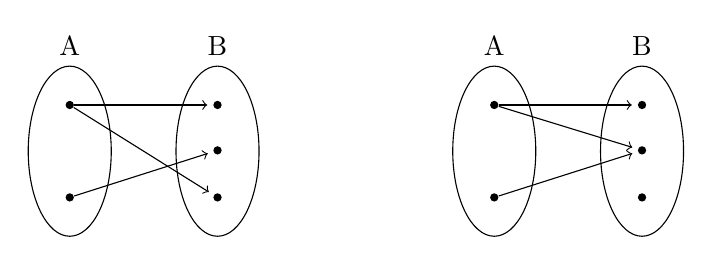
\begin{tikzpicture}
            [
            group/.style={ellipse, draw, minimum height=50pt,
                minimum width=30pt, label=above:#1},
            my dot/.style={circle, fill, minimum width=3pt, inner sep=0pt}
            ]
            \node (a) [my dot=a] {};
            \node (b) [below= 30pt of a, my dot=b] {};
            \node (c) [right=50pt of a, my dot=c] {};
            \node (d) [below= 13pt of c, my dot=d] {};
            \node (e) [right= 50pt of b, my dot=e] {};

            % Replicated nodes
            \node (a2) [right=150pt of a, my dot=a] {};
            \node (b2) [below=30pt of a2, my dot=b] {};
            \node (c2) [right=50pt of a2, my dot=c] {};
            \node (d2) [below=13pt of c2, my dot=d] {};
            \node (e2) [right=50pt of b2, my dot=e] {};

            \foreach \i/\j in {a/c,a/e,b/d}
            \draw [->, shorten >=2pt] (\i) -- (\j);
            \node [fit=(a) (b), group=A] {};
            \node [fit=(d) (c) (e), group=B] {};

            \foreach \i/\j in {a2/c2,a2/d2,b2/d2}
            \draw [->, shorten >=2pt] (\i) -- (\j);
            \node [fit=(a2) (b2), group=A] {};
            \node [fit=(d2) (c2) (e2), group=B] {};
        \end{tikzpicture}  

        \caption{\label{fig:figure1} Examples of functions.}
    \end{figure}

    \begin{figure}[H]
        \centering

        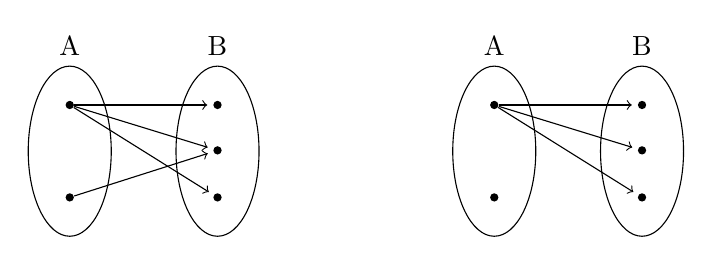
\begin{tikzpicture}
            [
            group/.style={ellipse, draw, minimum height=50pt, 
                minimum width=30pt, label=above:#1},
            my dot/.style={circle, fill, minimum width=3pt, inner sep=0pt}
            ]
            \node (a) [my dot=a] {};
            \node (b) [below= 30pt of a, my dot=b] {};
            \node (c) [right=50pt of a, my dot=c] {};
            \node (d) [below= 13pt of c, my dot=d] {};
            \node (e) [right= 50pt of b, my dot=e] {};

            % Replicated nodes
            \node (a2) [right=150pt of a, my dot=a] {};
            \node (b2) [below=30pt of a2, my dot=b] {};
            \node (c2) [right=50pt of a2, my dot=c] {};
            \node (d2) [below=13pt of c2, my dot=d] {};
            \node (e2) [right=50pt of b2, my dot=e] {};

            \foreach \i/\j in {a/c,a/e,b/d,a/d}
            \draw [->, shorten >=2pt] (\i) -- (\j);
            \node [fit=(a) (b), group=A] {};
            \node [fit=(d) (c) (e), group=B] {};

            \foreach \i/\j in {a2/c2,a2/d2,a2/e2}
            \draw [->, shorten >=2pt] (\i) -- (\j);
            \node [fit=(a2) (b2), group=A] {};
            \node [fit=(d2) (c2) (e2), group=B] {};
        \end{tikzpicture}  

        \caption{
            \label{fig:figure1} Examples of relations 
            that aren't functions.
        }
    \end{figure}
    
    A \textbf{binary operator} on a set $G$ is a function
    $f: G \times G \rightarrow G$.
    It takes in an ordered pair of elements from $G$ as input,
    and maps it to an element from the same set,
    matching the \textit{association} of the two elements to the output. \\
    Thus a binary operator maps $(a, b)$
    to an output $c$ $\forall a, b \in G$. \\
    We write $a \cdot b = c$ whenever we want to express that 
    $\cdot((a, b)) = c$. \\

    Suppose we chain binary operations,
    such as this one $a \cdot b \cdot c$.
    If $\forall a, b, c \in G$,
    the result does not depend on the order
    in which we resolve the operations,
    the binary operator is said to be \textbf{associative}. \\
    In other words, if $\cdot$ is associative,
    then
    $a \cdot b \cdot c = (a \cdot b) \cdot c = a \cdot (b \cdot c)$. \\
    For example,
    the $+$ operator applied on the set of integers $\Z$
    is associative. \\
    Note that the property of associativity
    applies for any number of operands,
    not just three.
    If a binary operator is associative with three operands,
    it has to be associative with any number of operands.
    Using induction,
    we will later show that the property holds for $n$ elements. \\

    A binary operator is said to be \textbf{commutative}
    if the order of the operands (not operations) does not affect
    the result of the operation as a whole.
    In other words, if $\forall a, b \in G$,
    $a \cdot b = b \cdot a$,
    we say $\cdot$ is commutative. \\
    For example,
    the $\times$ operator applied on the set of integers $\Z$
    is commutative,
    though the $\div$ operator is not. \\
    Again, this property implies that we can shift around operands
    regardless of how many operations we have chained.
    It can also be shown using induction. \\

    Given a binary operator $\cdot$ on $G$
    and a subset $H \subseteq G$,
    if $a \cdot b \in H$ for all $a, b \in H$,
    we say that the operator $\cdot$ is \textbf{closed} under $H$. \\
    For example,
    the $+$ operator applied on the set of integers $\Z$
    is closed under the set of positive integers $\Z^+$. \\
    Note that by our defintion of a binary operator,
    if the operator $\cdot$ is defined on the set $G$,
    it is always closed under $G$. \\
    

    \subsection*{Groups}

    A \textbf{group} is an ordered pair $(G, \cdot)$
    where $\cdot$ is a binary operator defined on $G$
    and the following axioms hold:
    \begin{itemize}[label=$\diamond$]
        \item 
            The binary operator must be associative.
        \item 
            There must be an element $e$ in $G$ called the \textbf{identity},
            such that $\forall a \in G$,
            $e \cdot a = a \cdot e = a$.
            Note that this implies $e$ commutes with all elements of $G$.
        \item
            For each element $a \in G$,
            there must be an element $a^{-1} \in G$,
            called the \textbf{inverse},
            such that $a \cdot a^{-1} = a^{-1} \cdot a = e$,
            the identity.
    \end{itemize}
    To give an example of a group,
    take $(\Z, +)$,
    the additive group of integers,
    where the inverse of element $a$ is it negation $-a$,
    and the identity is $0$. \\ 
    Note that other books sometimes also add a fourth axiom,
    stating that the binary operation must be closed under $G$.
    However, in this book, the property is built into the definition
    of the binary operator. \\

    The idea behind groups is the abstraction of objects.
    Instead of having, for instance,
    number that one can add and subtract and multiply,
    we can extend that defintion to any set and any operation,
    so long as it satisfies our definition. \\
    Furthermore,
    by focusing on the way a binary operation associates inputs
    with outputs in a set,
    we can abstract away the elements of a group and focus on its structure.
    This is useful for isolating mathematical characteristics of an object,
    and identifying similarities between objects. \\

    A group is said to be \textbf{abelian}
    if its binary operator is commutative,
    meaning that all of the elements in the group must commute. \\

    A group is finite if the set $G$ is finite. \\

    If we have two groups $(A, \cdot)$ and $(B, \diamond)$,
    we can form a new group $(A \times B, \circ)$,
    called their \textbf{direct product}.
    The operator $\circ$ of the group is defined on the cartesian product
    of the sets $A$ and $B$ as follows: \\ 
    For all elements $a_1, a_2 \in A$ and $b_1, b_2 \in B$,
    $(a_1, b_1) \circ (a_2, b_2) = (a_1 \cdot b_1, b_1 \diamond b_2)$. \\


    \subsection*{Properties of Groups}

    Before we begin,
    we note that for the rest of the section,
    unless specified otherwise,
    the group we are working in is assumed to be $(G, \cdot)$,
    with identity $e$. \\

    The identity of a group is unique.
    When we defined the identity of a group,
    we never specified that it had to be unique.
    Nevertheless,
    this property follows from the definition of the identity,
    and it can be proven. \\
    Suppose both $f$ and $g$ are identities of $G$.
    Since $f$ is an identity, we have that $f \cdot g = g$.
    Likewise, since $g$ is also identity, we have that $f \cdot g = f$.
    So $f = g$, proving that the identity is unique. \\

    For each element $a$ of a group, its inverse $a^{-1}$ is unqiue.
    Again, we did not define the inverse to be unique,
    but it follows all the same from its definition. \\
    Suppose that both $b$ and $c$ are inverses of $a$ in $G$.
    So $(b \cdot a) = e$, and $(a \cdot c) = e$
    By the associativity of $\cdot$, 
    we know that $(b \cdot a) \cdot c = b \cdot (a \cdot c)$.
    But that implies that $e \cdot c = b \cdot e$,
    which means that $c = b$.
    This proves the inverse is be unique. \\

    For any element $a$ of $G$, $(a^{-1})^{-1} = a$.
    This follows from the inverse's defintion,
    and the uniqueness of $a^{-1}$. \\
    We know by definition that $a \cdot a^{-1} = e$.
    We also know that $(a^{-1})^{-1} \cdot a^{-1} = e$.
    Since the inverse is unique,
    and both $(a^{-1})^{-1}$ and $a$ turn $a^{-1}$ into $e$,
    it must be that $(a^{-1})^{-1} = a$. \\

    For all elements $a$ and $b$ of $G$,
    $(a \cdot b)^{-1} = b^{-1} \cdot a^{-1}$. \\ 
    To prove this,
    suppose that $c = (a \cdot b)^{-1}$.
    As we showed earlier, the inverse of the inverse of an element
    is the element itself,
    so $c^{-1} = ((a \cdot b)^{-1})^{-1} = (a \cdot b)$. \\
    Since $c \cdot c^{-1} = e$,
    we can write that $c \cdot (a \cdot b) = e$. \\
    But by associativity,
    thus must mean that $(c \cdot a) \cdot b = e$. \\
    If we add $b^{-1}$ and $a^{-1}$ to both sides, we get
    \[(c \cdot a) \cdot b \cdot b^{-1} = e \cdot b^{-1}\]
    \[(c \cdot a) = b^{-1}\]
    \[(c \cdot a) \cdot a^{-1} = b^{-1} \cdot a^{-1} \]
    \[c \cdot (a \cdot a^{-1}) = b^{-1} \cdot a^{-1} \]
    \[c \cdot e = b^{-1} \cdot a^{-1} \]
    \[c = b^{-1} \cdot a^{-1} \]
    \[(a \cdot b)^{-1} = b^{-1} \cdot a^{-1} \]
    Completing the proof. \\

    In $G$, no matter how many element we chain together
    $a \cdot b \cdot c \cdot d \dots$,
    the result is independent of the bracketing.
    We already know that all binary operators in a group must be
    associative for three operands.
    However, it must also be noted
    that associativity with three operands
    implies \textbf{general associativity}. \\ 
    We can prove this using strong induction: \\
    \begin{adjustwidth}{1cm}{1cm} % Adjusts the left and right margins
        \textbf{Basis step:}
        For $n = 1$ and $n = 2$, we just have $a_1$ and $a_1 \cdot a_2$.
        For $n = 3$, we know that the group operation is always
        associative, such that $\forall a_1, a_2, a_3 \in G$,
        $(a_1 \cdot a_2) \cdot a_3 = a_1 \cdot (a_2 \cdot a_3)$. \\
        \textbf{Inductive hypothesis:}
        Assume that for $4 \leqslant n \leqslant k-1$,
        an arbitrarily bracketed expression
        $a_1 \cdot a_2 \cdot a_3 \dots a_n$
        always evaluates to 
        $a_1 \cdot (a_2 \cdot (a_3 \cdot (\dots (a_n))))$.
        Since all expression with $n$ operands evaluate to the same one,
        by transitivity, they must all evaluate to the same result. \\
        \textbf{Inductive step:}
        Assume that for $k$ operands,
        the expression $a_1 \cdot a_2 \cdot a_3 \dots a_k$
        is arbitrarily bracketed.
        We know that of the operators, one must have priority.
        Taking the two expression on either side of this operator,
        we get two arbitrarily bracketed expressions
        \[(a_1 \cdot a_2 \cdot a_3 \dots a_p)
        \cdot (a_{p+1} \cdot a_{p+2} \dots a_k)\]
        Since $p < k$,
        by our inductive hypothesis,
        the left side can be bracketed as wish without affecting its value,
        so we seperate out the first element,
        getting three expressions in the process.
        \[a_1 \cdot (a_2 \cdot a_3 \cdot a_4 \dots a_p)
        \cdot (a_{p+1} \cdot a_{p+2} \dots a_k)\]
        We can now consider the two terms to the right of $a_1$.
        \[a_1 \cdot ((a_2 \cdot a_3 \cdot a_4 \dots a_p)
        \cdot (a_{p+1} \cdot a_{p+2} \dots a_k))\]
        Together, they contain exactly $k-1$ elements.
        By the inductive hypothesis,
        we can bracket them however we please without changing their value.
        We can thus bracket them as such.
        \[a_1 \cdot ((a_2 \cdot a_3 \cdot ( \dots
        \cdot (a_k))))\]
    \end{adjustwidth}
    With that the proof is complete. \\


    \subsection*{Additional Notes}

    Instead of using $a \cdot b$ for an arbitrary operator,
    we will henceforth use $ab$.
    Likewise, instead of using $e$ for the identity, we will use $1$. \\ 
    We will also use $x^n$ to denote
    $\underbrace{x \cdot x \cdot ... x}_{n}$
    and $x^{-n}$ to denote
    $\underbrace{x^{-1} \cdot x^{-1} \cdot ... x^{-1}}_{n}$. \\

    The expression $ax = b$
    where $a, b, x \in G$ and $x$ is unknown
    has a single solution. \\ 
    This follows from the uniquess of the inverse,
    since adding $a^{-1}$ to both sides of the expression
    gives us $x = ba^{-1}$. \\

    By the same principle, $xa = ya$ implies that $x = y$. \\
    Again we can add the inverse of $a$
    to both sides to get the second expression. \\

    The \textbf{order} of a group $G$ is denoted by $|G|$,
    and it refers to the number of elements (cardinality) of the set $G$. \\
    For an infinite group, $|G| = \inf$. \\

    The order of an element $a \in G$, denoted by $|a|$,
    is the smallest value $n$ such that $a^n = 1$. \\
    If no such value exists, we say $a$ has infinite order. \\
    The identity $1$ is the only element with order $1$.
    This follows from the uniqueness of the identity. \\
    
    The \textbf{multiplicative table} of a group
    $G$ made up of the set $\{ 1, g_2, g_3, g_4 \dots g_n \}$
    is the $n \times n$ matrix $A$
    where any entry $a_{ij}$
    represents the value of $g_ig_j$. \\
    Such a table carries all the information of a group,
    and yet, is usually not very useful.
    For one, it is too large,
    and can't even be used with inifnite groups. \\
    \begin{figure}[H]
        \centering
        \[\vbox{\tabskip0.5em\offinterlineskip
        \halign{\strut$#$\hfil\ \tabskip1em\vrule&&$#$\hfil\cr
        ~   & 1   & g_2   & \dots & g_n \cr
        \noalign{\hrule}\vrule height 12pt width 0pt
        1   & 1 & g_2 & \dots & g_n \cr 
        g_2   & g_2 & g_2^2 & \dots & g_2g_n \cr 
        \vdots  & \vdots & \vdots & \ddots & \vdots \cr 
        g_n   & g_n & g_ng_2 & \dots & g_n^2 \cr
        }}\]
        \caption{\label{fig:figure1} The multiplicative table of $G$.}
    \end{figure}

\end{document}
